% Options for packages loaded elsewhere
\PassOptionsToPackage{unicode}{hyperref}
\PassOptionsToPackage{hyphens}{url}
\PassOptionsToPackage{dvipsnames,svgnames*,x11names*}{xcolor}
%
\documentclass[
  10pt,
  ignorenonframetext,
  x11names, dvipsnames, bibspacing,natbib]{beamer}
\usepackage{pgfpages}
\setbeamertemplate{caption}[numbered]
\setbeamertemplate{caption label separator}{: }
\setbeamercolor{caption name}{fg=normal text.fg}
\beamertemplatenavigationsymbolsempty
% Prevent slide breaks in the middle of a paragraph
\widowpenalties 1 10000
\raggedbottom
\setbeamertemplate{part page}{
  \centering
  \begin{beamercolorbox}[sep=16pt,center]{part title}
    \usebeamerfont{part title}\insertpart\par
  \end{beamercolorbox}
}
\setbeamertemplate{section page}{
  \centering
  \begin{beamercolorbox}[sep=12pt,center]{part title}
    \usebeamerfont{section title}\insertsection\par
  \end{beamercolorbox}
}
\setbeamertemplate{subsection page}{
  \centering
  \begin{beamercolorbox}[sep=8pt,center]{part title}
    \usebeamerfont{subsection title}\insertsubsection\par
  \end{beamercolorbox}
}
\AtBeginPart{
  \frame{\partpage}
}
\AtBeginSection{
  \ifbibliography
  \else
    \frame{\sectionpage}
  \fi
}
\AtBeginSubsection{
  \frame{\subsectionpage}
}
\usepackage{amsmath,amssymb}
\usepackage{lmodern}
\usepackage{ifxetex,ifluatex}
\ifnum 0\ifxetex 1\fi\ifluatex 1\fi=0 % if pdftex
  \usepackage[T1]{fontenc}
  \usepackage[utf8]{inputenc}
  \usepackage{textcomp} % provide euro and other symbols
\else % if luatex or xetex
  \usepackage{unicode-math}
  \defaultfontfeatures{Scale=MatchLowercase}
  \defaultfontfeatures[\rmfamily]{Ligatures=TeX,Scale=1}
\fi
\usetheme[]{Rafal_beamerSly1}
% Use upquote if available, for straight quotes in verbatim environments
\IfFileExists{upquote.sty}{\usepackage{upquote}}{}
\IfFileExists{microtype.sty}{% use microtype if available
  \usepackage[]{microtype}
  \UseMicrotypeSet[protrusion]{basicmath} % disable protrusion for tt fonts
}{}
\makeatletter
\@ifundefined{KOMAClassName}{% if non-KOMA class
  \IfFileExists{parskip.sty}{%
    \usepackage{parskip}
  }{% else
    \setlength{\parindent}{0pt}
    \setlength{\parskip}{6pt plus 2pt minus 1pt}}
}{% if KOMA class
  \KOMAoptions{parskip=half}}
\makeatother
\usepackage{xcolor}
\IfFileExists{xurl.sty}{\usepackage{xurl}}{} % add URL line breaks if available
\IfFileExists{bookmark.sty}{\usepackage{bookmark}}{\usepackage{hyperref}}
\hypersetup{
  pdftitle={Taking uncertainty in word embedding bias estimation seriously ~a Bayesian approach},
  pdfauthor={Alicja Dobrzeniecka \& Rafal Urbaniak (LoPSE research group, University of Gdansk)},
  colorlinks=true,
  linkcolor=Maroon,
  filecolor=Maroon,
  citecolor=Blue,
  urlcolor=blue,
  pdfcreator={LaTeX via pandoc}}
\urlstyle{same} % disable monospaced font for URLs
\newif\ifbibliography
\usepackage{longtable,booktabs,array}
\usepackage{calc} % for calculating minipage widths
\usepackage{caption}
% Make caption package work with longtable
\makeatletter
\def\fnum@table{\tablename~\thetable}
\makeatother
\setlength{\emergencystretch}{3em} % prevent overfull lines
\providecommand{\tightlist}{%
  \setlength{\itemsep}{0pt}\setlength{\parskip}{0pt}}
\setcounter{secnumdepth}{-\maxdimen} % remove section numbering
\ifluatex
  \usepackage{selnolig}  % disable illegal ligatures
\fi
\newlength{\cslhangindent}
\setlength{\cslhangindent}{1.5em}
\newlength{\csllabelwidth}
\setlength{\csllabelwidth}{3em}
\newenvironment{CSLReferences}[2] % #1 hanging-ident, #2 entry spacing
 {% don't indent paragraphs
  \setlength{\parindent}{0pt}
  % turn on hanging indent if param 1 is 1
  \ifodd #1 \everypar{\setlength{\hangindent}{\cslhangindent}}\ignorespaces\fi
  % set entry spacing
  \ifnum #2 > 0
  \setlength{\parskip}{#2\baselineskip}
  \fi
 }%
 {}
\usepackage{calc}
\newcommand{\CSLBlock}[1]{#1\hfill\break}
\newcommand{\CSLLeftMargin}[1]{\parbox[t]{\csllabelwidth}{#1}}
\newcommand{\CSLRightInline}[1]{\parbox[t]{\linewidth - \csllabelwidth}{#1}\break}
\newcommand{\CSLIndent}[1]{\hspace{\cslhangindent}#1}

\title{\large Taking uncertainty in word embedding bias estimation
seriously ~a Bayesian approach}
\author{Alicja Dobrzeniecka \& Rafal Urbaniak
\footnotesize \newline (LoPSE research group, University of Gdansk)}
\date{ExpSem2021, ESSLLI}

\begin{document}
\frame{\titlepage}

\begin{frame}{Cosine-based measures of bias}
\protect\hypertarget{cosine-based-measures-of-bias}{}
\begin{block}{Word embeddings}
\protect\hypertarget{word-embeddings}{}
\begin{itemize}
\item
  Representation of words (or words in contexts) with vectors of real
  numbers
\item
  Built to predict the probability of co-occurence
\end{itemize}

\begin{longtable}[]{@{}llllll@{}}
\toprule
word & 1 & 2 & 3 & 4 & \ldots{} \\
\midrule
\endhead
woman & 0.456 & 0.267 & 0.675 & 0.131 & \ldots{} \\
man & 0.451 & 0.897 & 0.472 & 0.088 & \ldots{} \\
\bottomrule
\end{longtable}
\end{block}
\end{frame}

\begin{frame}{Cosine-based measures of bias}
\protect\hypertarget{cosine-based-measures-of-bias-1}{}
\begin{block}{Cosine similarity \& distance}
\protect\hypertarget{cosine-similarity-distance}{}
\vspace{-4mm}

\begin{align} \tag{Sim}
\mathsf{cosineSimilarity}(A,B) & = \frac{A \cdot B}{\vert \vert A \vert \vert \,\vert \vert B \vert \vert}
\\
\tag{Distance}
\mathsf{cosineDistance}(A,B) &  = 1 - \mathsf{cosineSimilarity}(A,B)
\end{align}

\begin{itemize}
\item
  Geometric interpretation: direction (not length)
\item
  \(\mathsf{cosineDistance}\in (0, 2)\)
\item
  Naive interpretation: proximity corresponds to semantic similarity
  (e.g.~no triangle inequality)
\end{itemize}
\end{block}
\end{frame}

\begin{frame}{Cosine-based measures of bias}
\protect\hypertarget{cosine-based-measures-of-bias-2}{}
\begin{block}{The worry}
\protect\hypertarget{the-worry}{}
In the learning process these models can learn implicit biases that
reflect harmful stereotypical thinking

\pause
\end{block}

\begin{block}{Cosine-based bias: basic intuition}
\protect\hypertarget{cosine-based-bias-basic-intuition}{}
Words belonging to an intuitively harmful stereotype are cosine-close to
each other
\end{block}
\end{frame}

\begin{frame}{Cosine-based measures of bias}
\protect\hypertarget{cosine-based-measures-of-bias-3}{}
\begin{block}{Stereotypical lists}
\protect\hypertarget{stereotypical-lists}{}
\footnotesize

\begin{itemize}
\item
  feminine occupations: ``homemaker,'' ``nurse,'' ``receptionist,''
  ``librarian,'' etc.
\item
  masculine occupations: ``maestro,'' ``captain,'' ``architect,'' etc.
\end{itemize}

\normalsize
\end{block}

\begin{block}{Visual example}
\protect\hypertarget{visual-example}{}
\vspace{1mm}
\footnotesize

\begin{center}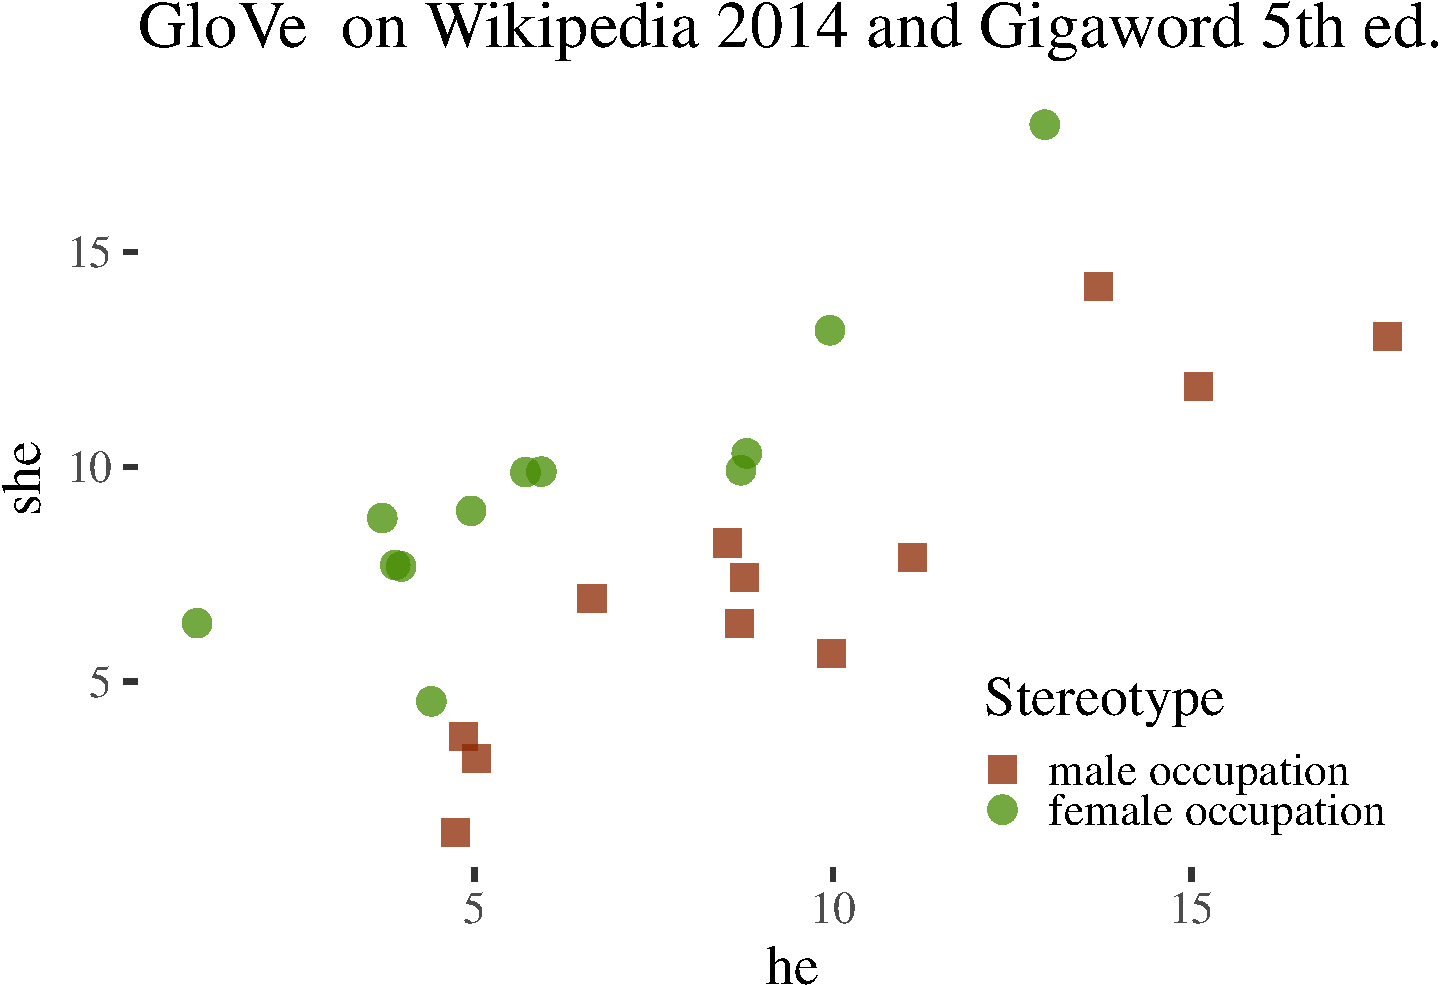
\includegraphics[width=0.6\linewidth]{presentationESSLLI_files/figure-beamer/unnamed-chunk-1-1} \end{center}
\normalsize
\end{block}
\end{frame}

\begin{frame}{Cosine-based measures of bias}
\protect\hypertarget{cosine-based-measures-of-bias-4}{}
\begin{block}{Example: direct bias}
\protect\hypertarget{example-direct-bias}{}
\begin{itemize}
\tightlist
\item
  The gender bias of a word \(w\) is its projection on the gender
  direction
  \(\vec{w} \cdot (\overrightarrow{he} - \overrightarrow{she})\)
\end{itemize}

\begin{itemize}
\tightlist
\item
  Given the (ideally) gender neutral words \(N\) and the gender
  direction \(g\) the direct gender bias is:
\end{itemize}

\vspace{-2mm}

\begin{align}
\mathsf{directBias_c(N,g)} & = \frac{\sum_{w\in N}\vert \mathsf{cos}(\vec{w},g)\vert^c}{\vert N \vert }
\end{align}

\footnotesize

(\protect\hyperlink{ref-Bolukbasi2016Man}{Bolukbasi, Chang, Zou,
Saligrama, \& Kalai, 2016})
\end{block}
\end{frame}

\begin{frame}{Cosine-based measures of bias}
\protect\hypertarget{cosine-based-measures-of-bias-5}{}
\begin{block}{Example: Word Embedding Association Test (WEAT)}
\protect\hypertarget{example-word-embedding-association-test-weat}{}
\begin{align*}
s(t,A,B) & = \frac{\sum_{a\in A}f(t,a)}{\vert A\vert} - \frac{\sum_{b\in B}f(t,b)}{\vert B\vert}
\\
WEAT(A,B) & = \frac{
\mu\left(\{s(x,A,B)\}_{x\in X}\right) -\mu\left(\{s(y,A,B)\}_{y\in Y}\right) 
}{
\sigma\left(\{s(w,A,B)\}_{w\in X\cup Y}\right)
}
\end{align*}

\begin{itemize}
\item
  \(t\) is a term, \(A, B\) are sets of stereotype attribute words, \$X,
  \(Y\) are protected group words
\item
  For instance, \(X\) might be a set of male names, \(Y\) a set of
  female names, \(A\) might contain stereotypically male-related career
  words, and \(B\) stereotypically female-related family words
\item
  \(s\)-values are used as datapoints in statistical significance tests
\end{itemize}

\footnotesize

(\protect\hyperlink{ref-Caliskan2017semanticsBiases}{Caliskan, Bryson,
\& Narayanan, 2017}) with extensions in
(\protect\hyperlink{ref-Lauscher2019multidimensional}{Lauscher \&
Glavas, 2019}) and applications in
(\protect\hyperlink{ref-Garg2018years}{Garg, Schiebinger, Jurafsky, \&
Zou, 2018})
\end{block}
\end{frame}

\begin{frame}{Cosine-based measures of bias}
\protect\hypertarget{cosine-based-measures-of-bias-6}{}
\begin{block}{Our main target: Mean Average Cosine Similarity (MAC)}
\protect\hypertarget{our-main-target-mean-average-cosine-similarity-mac}{}
\begin{align*}
S(t_i, A_j) & = \frac{1}{\vert A_j\vert}\sum_{a\in A_j}\mathsf{cos}(t,a) \\
MAC(T,A) & = \frac{1}{\vert T \vert \,\vert A\vert}\sum_{t_i \in T }\sum_{A_j \in A} S(t_i,A_j)
\end{align*}

\begin{itemize}
\item
  \(T = \{t_1, \dots, t_k\}\) is a class of protected words
\item
  each \(A_j\in A\) is a set of attributes stereotypically associated
  with a protected word
\end{itemize}

\begin{itemize}
\tightlist
\item
  The t-tests they employ are run on average cosines used to calculate
  MAC
\end{itemize}

\footnotesize

(\protect\hyperlink{ref-Manzini2019blackToCriminal}{Manzini, Lim,
Tsvetkov, \& Black, 2019})
\end{block}
\end{frame}

\begin{frame}{Cosine-based measures of bias}
\protect\hypertarget{cosine-based-measures-of-bias-7}{}
\begin{block}{Our main target: Mean Average Cosine Similarity (MAC)}
\protect\hypertarget{our-main-target-mean-average-cosine-similarity-mac-1}{}
\footnotesize 
\begin{table}

\caption{\label{tab:religionTableHeadEarly}Rows the religion dataset.}
\centering
\resizebox{\linewidth}{!}{
\begin{tabular}[t]{llrr}
\toprule
protectedWord & wordToCompare & cosineDistance & cosineSimilarity\\
\midrule
jew & greedy & 0.6947042 & 0.3052958\\
rabbi & greedy & 1.0306175 & -0.0306175\\
rabbi & conservative & 0.7175887 & 0.2824113\\
christian & uneducated & 0.5081939 & 0.4918061\\
christianity & cheap & 1.2816164 & -0.2816164\\
muslim & terrorist & 0.2726106 & 0.7273894\\
\bottomrule
\end{tabular}}
\end{table}
\normalsize
\end{block}
\end{frame}

\begin{frame}{Cosine-based measures of bias}
\protect\hypertarget{cosine-based-measures-of-bias-8}{}
\begin{block}{Known challenges}
\protect\hypertarget{known-challenges}{}
\begin{itemize}
\item
  Gender-direction might be an indicator of bias, but is insufficient.
  After debiasing other non-gendered words can remain in biased
  relations (\protect\hyperlink{ref-Gonen2019lipstick}{Gonen \&
  Goldberg, 2019})
\item
  Methods which involve analogies and their evaluations by human users
  on Mechanical Turk are unreliable
  (\protect\hyperlink{ref-Nissim2020fair}{Nissim, Noord, \& Goot, 2020})
\end{itemize}
\end{block}
\end{frame}

\begin{frame}{Some methodological problems}
\protect\hypertarget{some-methodological-problems}{}
\begin{block}{Word list choice is unprincipled}
\protect\hypertarget{word-list-choice-is-unprincipled}{}
We run with it for comparison

\pause
\end{block}

\begin{block}{No design considerations to sample size}
\protect\hypertarget{no-design-considerations-to-sample-size}{}
We investigate the uncertainty that arises from raw sample sizes
\end{block}
\end{frame}

\begin{frame}{Some methodological problems}
\protect\hypertarget{some-methodological-problems-1}{}
\begin{block}{No word class distinction and no control group}
\protect\hypertarget{no-word-class-distinction-and-no-control-group}{}
We make the subclasses clear, add human neutral predicates and neutral
predicates for control

\footnotesize 
\begin{table}

\caption{\label{tab:religionTableHeadLate}Rows from extended religion dataset.}
\centering
\resizebox{\linewidth}{!}{
\begin{tabular}[t]{lllrrl}
\toprule
protectedWord & wordToCompare & wordClass & cosineDistance & cosineSimilarity & connection\\
\midrule
torah & hairy & jewish & 1.170 & -0.170 & associated\\
christian & dirty & muslim & 0.949 & 0.051 & different\\
judaism & cheap & jewish & 1.232 & -0.232 & associated\\
christianity & familial & christian & 0.645 & 0.355 & associated\\
mosque & approve & neutral & 0.995 & 0.005 & none\\
imam & carry & human & 0.993 & 0.007 & human\\
mosque & merging & neutral & 0.868 & 0.132 & none\\
muslim & nationalized & neutral & 0.870 & 0.130 & none\\
\bottomrule
\end{tabular}}
\end{table}
\normalsize
\end{block}
\end{frame}

\begin{frame}{Some methodological problems}
\protect\hypertarget{some-methodological-problems-2}{}
\begin{block}{Outliers and surprisingly dissimilar words}
\protect\hypertarget{outliers-and-surprisingly-dissimilar-words}{}
We study those by visualizations and uncertainty estimates

\pause
\end{block}

\begin{block}{No principled interpretation}
\protect\hypertarget{no-principled-interpretation}{}
\begin{longtable}[]{@{}ll@{}}
\toprule
Religion Debiasing & MAC (distance) \\
\midrule
\endhead
Biased & 0.859 \\
Hard Debiased & 0.934 \\
Soft Debiased (\(\lambda\) = 0.2) & 0.894 \\
\bottomrule
\end{longtable}

What values are sufficient for the presence of bias and what differences
are sign of real improvement? Low \(p\)-values are not high effect
indicators!

We compare HPDIs.
\end{block}
\end{frame}

\begin{frame}{The problem with pre-averaging}
\protect\hypertarget{the-problem-with-pre-averaging}{}
\begin{itemize}
\tightlist
\item
  It throws away information about sample sizes
\item
  It removes variation which may result in false confidence
\end{itemize}
\end{frame}

\begin{frame}{Cosine distance and word connection visualization}
\protect\hypertarget{cosine-distance-and-word-connection-visualization}{}
\begin{block}{Analysis of word ``muslim''}
\protect\hypertarget{analysis-of-word-muslim}{}
\begin{center}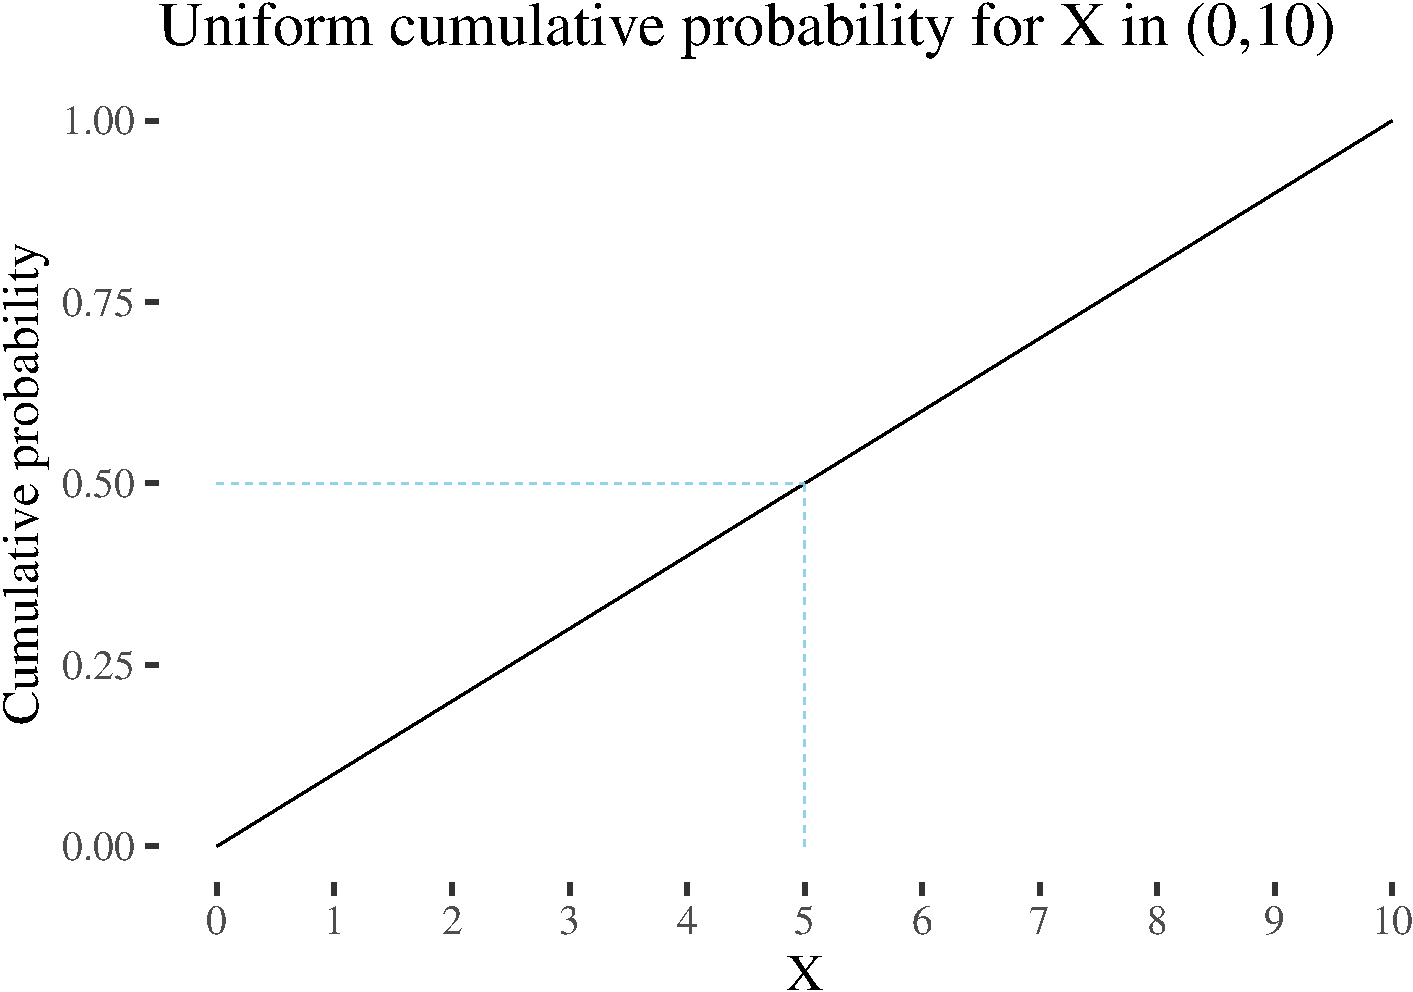
\includegraphics[width=1.05\linewidth]{presentationESSLLI_files/figure-beamer/unnamed-chunk-2-1} \end{center}
\end{block}
\end{frame}

\begin{frame}{Cosine distance and word connection visualization}
\protect\hypertarget{cosine-distance-and-word-connection-visualization-1}{}
\begin{block}{Analysis of word ``priest''}
\protect\hypertarget{analysis-of-word-priest}{}
\begin{center}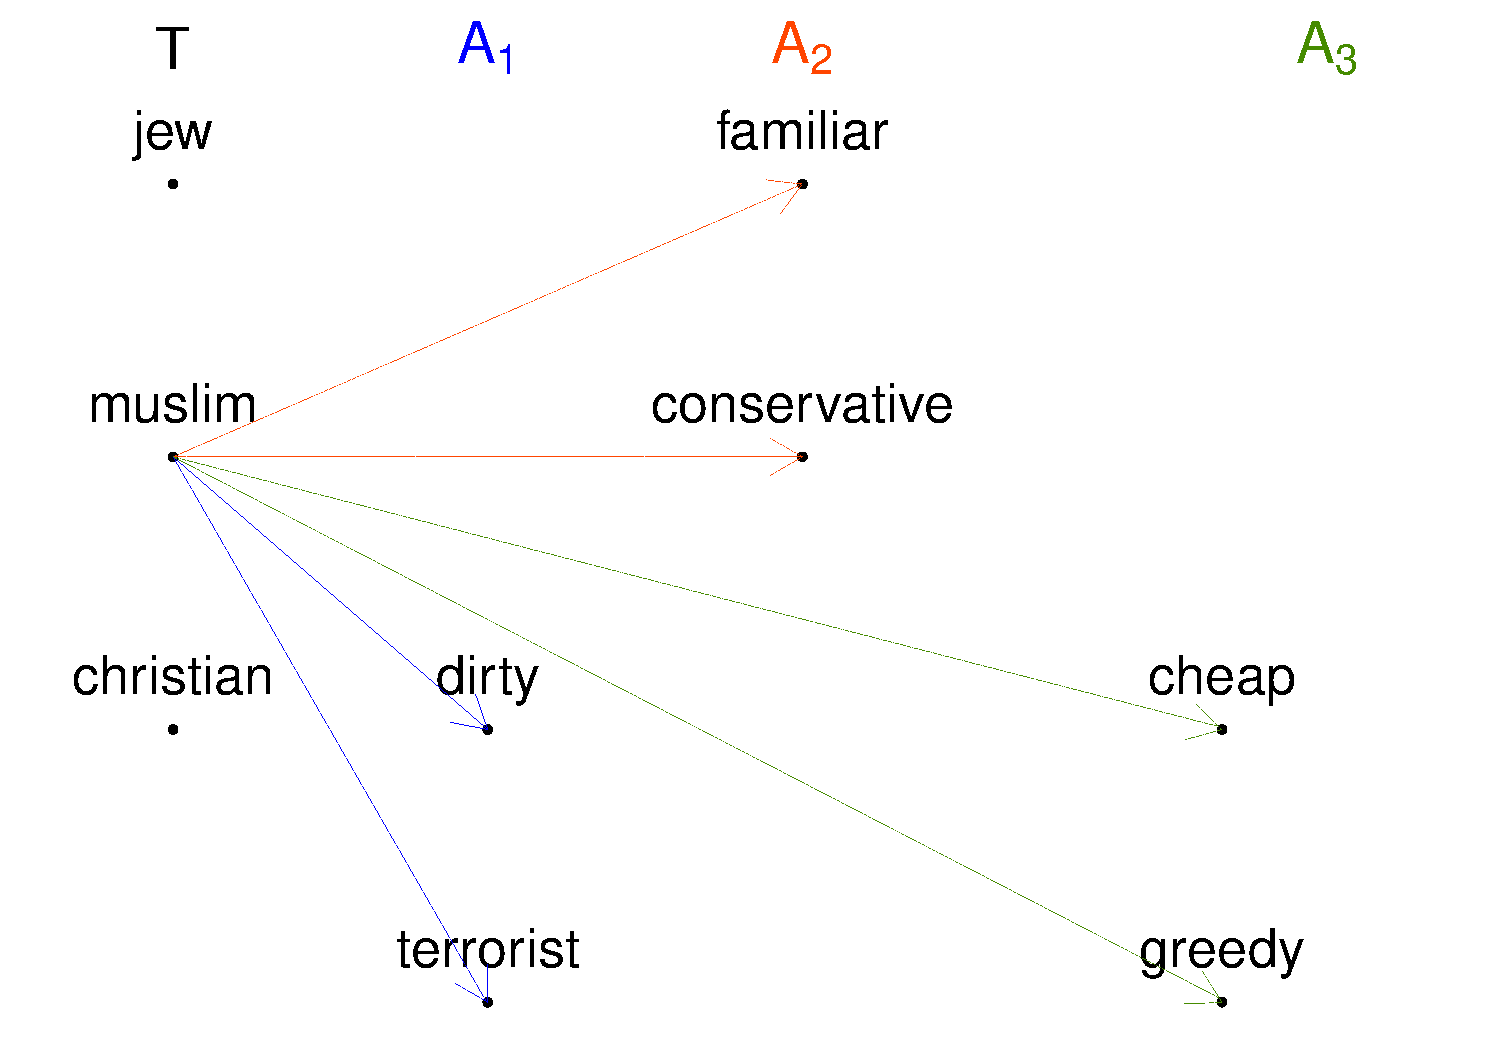
\includegraphics[width=1.05\linewidth]{presentationESSLLI_files/figure-beamer/unnamed-chunk-3-1} \end{center}
\end{block}
\end{frame}

\begin{frame}{Bayesian model}
\protect\hypertarget{bayesian-model}{}
\end{frame}

\begin{frame}{HPDIs}
\protect\hypertarget{hpdis}{}
\begin{block}{Further work}
\protect\hypertarget{further-work}{}
\begin{itemize}
\tightlist
\item
  downstream tasks
\end{itemize}
\end{block}
\end{frame}

\begin{frame}{References}
\protect\hypertarget{references}{}
\tiny

\hypertarget{refs}{}
\begin{CSLReferences}{1}{0}
\leavevmode\hypertarget{ref-Bolukbasi2016Man}{}%
Bolukbasi, T., Chang, K.-W., Zou, J. Y., Saligrama, V., \& Kalai, A.
(2016). Man is to computer programmer as woman is to homemaker?
Debiasing word embeddings. \emph{CoRR}, \emph{abs/1607.06520}. Retrieved
from \url{http://arxiv.org/abs/1607.06520}

\leavevmode\hypertarget{ref-Caliskan2017semanticsBiases}{}%
Caliskan, A., Bryson, J. J., \& Narayanan, A. (2017). Semantics derived
automatically from language corpora contain human-like biases.
\emph{Science}, \emph{356}(6334), 183--186.
\url{https://doi.org/10.1126/science.aal4230}

\leavevmode\hypertarget{ref-Garg2018years}{}%
Garg, N., Schiebinger, L., Jurafsky, D., \& Zou, J. (2018). Word
embeddings quantify 100 years of gender and ethnic stereotypes.
\emph{Proceedings of the National Academy of Sciences}, \emph{115}(16),
E3635--E3644. \url{https://doi.org/10.1073/pnas.1720347115}

\leavevmode\hypertarget{ref-Gonen2019lipstick}{}%
Gonen, H., \& Goldberg, Y. (2019). Lipstick on a pig: {D}ebiasing
methods cover up systematic gender biases in word embeddings but do not
remove them. \emph{Proceedings of the 2019 Conference of the North
{A}merican Chapter of the Association for Computational Linguistics:
Human Language Technologies, Volume 1 (Long and Short Papers)},
609--614. Minneapolis, Minnesota: Association for Computational
Linguistics. \url{https://doi.org/10.18653/v1/N19-1061}

\leavevmode\hypertarget{ref-Lauscher2019multidimensional}{}%
Lauscher, A., \& Glavas, G. (2019). Are we consistently biased?
Multidimensional analysis of biases in distributional word vectors.
\emph{CoRR}, \emph{abs/1904.11783}. Retrieved from
\url{http://arxiv.org/abs/1904.11783}

\leavevmode\hypertarget{ref-Manzini2019blackToCriminal}{}%
Manzini, T., Lim, Y. C., Tsvetkov, Y., \& Black, A. W. (2019).
\emph{Black is to criminal as caucasian is to police: Detecting and
removing multiclass bias in word embeddings}. Retrieved from
\url{http://arxiv.org/abs/1904.04047}

\leavevmode\hypertarget{ref-Nissim2020fair}{}%
Nissim, M., Noord, R. van, \& Goot, R. van der. (2020). Fair is better
than sensational: Man is to doctor as woman is to doctor.
\emph{Computational Linguistics}, \emph{46}(2), 487--497.
\url{https://doi.org/10.1162/coli_a_00379}

\end{CSLReferences}
\end{frame}

\end{document}
